
\begin{figure*}
\centering
%\centering
%\begin{tabular}{cc}
%\bmvaHangBox{\fbox{
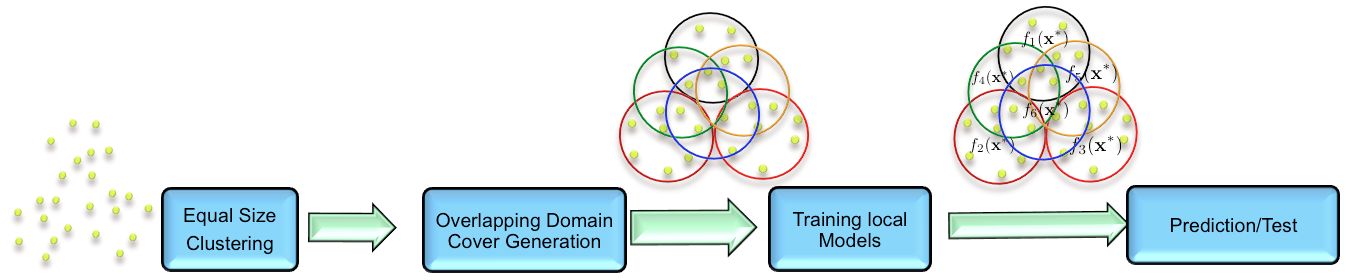
\includegraphics[width=1.0\textwidth]{method.png}
\caption{ODC Framework}
\end{figure*}

The problems of the existing approaches, presented 
above, motivated us to develop an approach that  satisfies the properties listed in  table~\ref{tbl:contr}.\ignore{(a) accurate, (b) efficient, (c) scalable to arbitrary input dimension and also consider structured output, (d) consistent on boundary predictions (i.e., no discontinuity problem) (e) applicable to various kernel machines, and (f) easy to parallelize; } The table also shows which of these properties are satisfied for the relevant methods.\ignore{For example, looking at Park's approach \cite{park11},  it satisfies properties (a), (d), and
(f) but not properties (b) and (c).\ignore{ Property (b) is satisfied when the approach is applied to small dimensional input. Hence, property (c) is not satisfied.} Similarly, the likelihood approximation methods like FIC~\cite{fic06} and PIC~\cite{pic07}),  have properties (e) and (c) not satisfied, and (d) not applicable. Chalupka et al~\cite{Chalupka:2013}'s local method has properties (a), (c) and (d) not satisfied. Finally, the  NN-local regression scheme does not satisfy (b).}
 \ignore{
 GPR, TGP and IWTGP require inversion of $N \times N$ matrices, so the complexity of the solution is $O(N^3)$ which is impractical when $N$ is large. However, some approaches was designed to resolve this problem in GPR (e.g. FIC \cite{fic06}, PIC \cite{pic07}), that suffer from difficulty of parallelism. Furthermore, they were prominently addressed in GPR, which predict single dimension output and has been outperformed by structured regression approached like TGP. Practically, TGP \cite{Bo:2010} approach has been applied by finding the $N' << N$ nearest neighbors.  Then the prediction is done by minimizing equation ~\ref{eq:tgp} in $O(N'^3)$ operations (because of the inversion of $N' \times N'$ matrices). \ignore{$N'$ was chosen to be ($N' \approx 800$)}.  Similarity, IWTGP \cite{Yamada:2012} requires matrix inversions of $N' \times N'$ matrices, the complexity of solving equation ~\ref{eq:IWTGP}. IWTGP also includes the estimation of relative importance weight, thus the total complexity of IWTGP is  $O({N'}^3)+ O({N'}_{tst}^3)$. However computing  the nearest neighbors is one way to tackle the performance problem but it has three drawbacks. (1) A TGP /IWTGP model is computed for each query point $x$, which results in a scalability  problems in prediction (i.e. Matrix inversions on the nearest neighbor of each each test point) (2) Number of neighbors might not be large enough to create an accurate prediction model since it is constrained by the first drawback. These drawbacks are overcome as a consequence of the six desirable properties (see section ~\ref{sec:1}), which are  satisfied by our overlapping set cover framework. We denote this nearest neighbor variants of GPR, TGP and IWTGP as GPR-KNN, TGP-KNN, and IWTGP-KNN respectively.} In order to satisfy all the properties, we \ignore{\begin{wraptable}{r}{7.7cm} \vspace{-4mm}\caption{Contrast against most relevant methods}
 \vspace{3mm}
  \label{tbl:contr}
\scalebox{0.53}
{
\begin{tabular}{|l|c|c|c|c|}
\hline 
  &\cite{park11} & FIC/PIC~\cite{fic06}& NN~\cite{Bo:2010} & ODC \\ 
\hline 
Accurate & \begin{tabular}{@{}c@{}}No for  high  \\ input dimension \end{tabular}  & No & Yes& Yes \\ 
\hline 
Efficient & No & Yes & No &  Yes\\ 
\hline 
\begin{tabular}{@{}c@{}}Scalable to arbitrary \\ input dimension \end{tabular}  & No (2D) & Yes & Yes& Yes \\ 
\hline 
Consistent on Boundaries & Yes & No & Yes & Yes \\ 
\hline 
supported kernel machines &GPR& GPR & TGP & GPR, TGP, IWTGP and others\\ 
\hline 
Easy to parallelize & No & No & Yes& Yes \\ 
\hline 
\end{tabular} 
}\vspace{-3mm}\end{wraptable}} present the Overlapping Domain Cover (ODC) notion. We define the ODC as a collection of overlapping subsets of the training points, denoted by  subdomains,  such that they are as spatially coherent as possible.\ignore{In order to achieve this objective, we model our framework as follows} During training, an ODC is computed such that each subdomain overlaps with the neighboring subdomains. Then, a  local prediction model (kernel machine) is \ignore{ \begin{wrapfigure}{r}{0.45\textwidth}
  \vspace{-12pt}
    \includegraphics[width=0.45\textwidth]{systemArch3.png}
  \caption{Overlapping Domain Cover Framework, applied to 3D pose instances taken from Human Eva dataset \cite{SigalBB10} }
  \label{fig:DDTGP}
%\label{fig:teaser}
  \vspace{-15pt}
\end{wrapfigure}} created for each subdomain and the computations that does not depend on the test data are factored out and precomputed (e.g. inversion of matrices). The nature of the ODC generation makes these kernel machines consistent in the overlapped regions, which are the boundaries since we constraint the subdomains to be coherent. This is motivated by the notion that data lives on a manifold with local properties and consistent connections between its neighboring regions. On prediction, the output is calculated as a reduction function of the predictions on the closed subdomain(s). Table~\ref{tab:thcomp}\ignore{, we show the computational complexity on testing and training including clustering if applicable using our parametrization and notations, i.e., as a function of $M$, $N$, $d_X$, and $d_Y$. The first row  shows the computational complexity for using full data and NN local regression scheme,  applied to either TGP or GPR. The third and the fourth rows show the complexity of FIC and Local-RPC applied to GPR in ~ and  ~\cite{Chalupka:2013} respectively.} ( the last row) shows the complexity for our generalized ODC framework, detailed in Sec~\ref{sec:4} and ~\ref{sec:pred}. In contrast to the prior work, our ODC framework is designed to cover structured regression setting, $d_Y>1$ and to be applicable to GPR, TGP, and many other models.\ignore{Having computed the ODC, a local kernel machine is trained on each member of the cover, denoted as subdomains. At test time, the  local kernel machines of the closest subdomains to the test point are retrieved and the final output is computed as a combination of their predictions.}

\begin{table}[t!] 
\caption{Contrast against most relevant methods}
  \label{tbl:contr}
\scalebox{0.68}
{
\begin{tabular}{|l|c|c|c|c|}
\hline 
  &\cite{park11} & FIC/PIC~\cite{fic06}& NN~\cite{Bo:2010} & ODC \\ 
\hline 
Accurate & \begin{tabular}{@{}c@{}}No for  high  \\ input dimension \end{tabular}  & No & Yes& Yes \\ 
\hline 
Efficient & No & Yes & No &  Yes\\ 
\hline 
\begin{tabular}{@{}c@{}}Scalable to arbitrary \\ input dimension \end{tabular}  & No (2D) & Yes & Yes& Yes \\ 
\hline 
Consistent on Boundaries & Yes & No & Yes & Yes \\ 
\hline 
supported kernel machines &GPR& GPR & TGP & GPR, TGP, IWTGP and others\\ 
\hline 
Easy to parallelize & No & No & Yes& Yes \\ 
\hline 
\end{tabular} 
}\end{table}
%
%\begin{table}[b!]
%\centering
%\begin{minipage}{0.6\textwidth}
%\centering
% \caption{Contrast against most relevant methods}
% \vspace{3mm}
%  \label{tbl:contr}
%\scalebox{0.53}
%{
%\begin{tabular}{|l|c|c|c|c|}
%\hline 
%  &\cite{park11} & FIC/PIC & NN & ODC \\ 
%\hline 
%Accurate & \begin{tabular}{@{}c@{}}No for  high  \\ input dimension \end{tabular}  & No & Yes& Yes \\ 
%\hline 
%Efficient & No & Yes & No &  Yes\\ 
%\hline 
%\begin{tabular}{@{}c@{}}Scalable to arbitrary \\ input dimension \end{tabular}  & No (2D) & Yes & Yes& Yes \\ 
%\hline 
%Consistent on Boundaries & Yes & No & Yes & Yes \\ 
%\hline 
%supported kernel machines &GPR& GPR & TGP & GPR, TGP, IWTGP and others\\ 
%\hline 
%Easy to parallelize & No & No & Yes& No \\ 
%\hline 
%\end{tabular} 
%}
%\end{minipage}
%\begin{minipage}{0.39\textwidth}
%\centering
%\captionof{figure}{AB-EKmeans on 300,000 2D points, K= 57}
%\label{figABkmeans57}
% \vspace{2mm}
%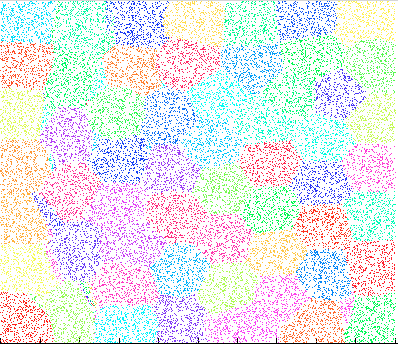
\includegraphics[width=2.8cm]{Ekmeans57.png}
%\end{minipage}
%\vspace{-5mm}
%\end{table}
 
%\begin{table}[b!]
%  %\vspace{-2mm}
%\centering
%  \caption{Contrast against most relevant methods}
%  \label{tbl:contr}
%\scalebox{0.53}
%{
%\begin{tabular}{|l|c|c|c|c|}
%\hline 
%  &\cite{park11} & FIC/PIC & NN & ODC \\ 
%\hline 
%Accurate & \begin{tabular}{@{}c@{}}No for  high  \\ input dimension \end{tabular}  & No & Yes& Yes \\ 
%\hline 
%Efficient & No & Yes & No &  Yes\\ 
%\hline 
%\begin{tabular}{@{}c@{}}Scalable to arbitrary \\ input dimension \end{tabular}  & No (2D) & Yes & Yes& Yes \\ 
%\hline 
%Consistent on Boundaries & Yes & No & Yes & Yes \\ 
%\hline 
%supported kernel machines &GPR& GPR & TGP & GPR, TGP, IWTGP and others\\ 
%\hline 
%Easy to parallelize & No & No & Yes& No \\ 
%\hline 
%\end{tabular} 
%}
%%\vspace{-3.8mm}
%\end{table}
\ignore{
The main intuition behind the ODC framework is to } \ignore{ create subdomains with optimized  consistency of prediction on the boundaries and }\ignore{increase the likelihood of finding a local kernel machine trained in a sufficient neighborhood of an arbitrary test point. {The framework is also motivated by the notion that \ignore behind this procedure is that }Data lives on a manifold, which has local properties and consistent connections between its neighboring subdomains. As a result, our framework is to model the problem as finding/learning these subdomains such that they have consistent predictions as possible, which is achieved by building overlapping kernel machines}\ignore{; Figure ~\ref{fig:DDTGP} shows the block diagram of our method, applied to 3D pose estimation as a regression problem.} 

\noindent\textbf{Notations.} Given a set of input data  $X=\{\mathbf{x}_1, \cdots, \mathbf{x}_N  \}$, our prediction framework firstly  generates a set of non-overlapping equal-size partitions,  $C=\{C_1, \cdots, C_K\}$, such that $\cup_{i}{C}_i = X$, $| C_i| = N/K$. Then, the ODC is defined based on them as $\mathcal{D} =  \{ {D}_1, \cdots, {D}_K \}$, such that $|{D}_i| =M\, \forall i$, ${D}_i = C_i \cup O_i, \forall i$\ignore{ is defined based on them, such that  }. $O_i$ a the set of points that overlaps with the other partitions, i.e.,  $O_i  = \{x: x \in  \{\cup_{j \neq i} {C}_j\} \}$,  such that $|O_i| = p \cdot M$, $|C_i| = (1-p) \cdot M$,   $0 \le p \le 1$ is the ratio of points in each overlapping subdomain, $D_i$, that belongs to/overlaps with partitions, other than its own, $C_i$. 

It is important to note that, the ODC could be specified by two parameters, $M$  and $p$, which are the number of points in each subdomain and the ratio of overlap respectively; this is since $K= N/ (1-p) M$.  This parameterization of ODC generation is reasonable for the following reasons. First, $M$ defines the number of points that are used to train each local kernel machine, which controls the performance of the local prediction. Second, given $M$ and that $K= N/ (1-p) M$, $p$  defines how coarse/fine the distribution of kernel machines are.  It is not hard to see that as $p$ goes to $0$, the generated ODC reduces to the set of non-overlapping clusters. Similarly, as $p$ approaches $1 - 1/M$, the ODC reduces to generating a cluster at each point with maximum overlap with other clusters, i.e., $K=N$, $|C_i|=1$, and $|O_i| = M -1$. 
\textit{Our main claim is two fold. First, precomputing local kernel machines (e.g.  GPR, TGP, IWTGP) during training on the ODC significantly increase the speedup on prediction time. Second, given a fixed $M$ and $N$, as $p$ increases, local prediction performance increases, theoretically supported by Lemma~\ref{lemma1}} 
\vspace{-0.5mm}
\begin{lem}
Under ODC notion, as the overlap $p$ increases, the  closer the nearest model to an arbitrary test point and the more likely that model get trained on a big neighborhood of the test point.  
\label{lemma1}
\end{lem}

\begin{proof}
We start by outlining the main idea behind  the proof, which is directly connected to the fact that $K= N/ (1-p) M$, which indicates that the number of local models increases as $p$ increases given fixed $N$ and $M$.  Under the assumption that the local models are spatially cohesive,  $p \to 1$ theoretically indicates that there is a local model  centered at each point in the space (\ie $K = \infty$). Hence, as $p$ increases, the distribution of the kernel machines is the finest and the more likely a test point to find the closest kernel machines trained on a big neighborhood of it leading to more accurate prediction. Meanwhile, as $p$ goes to $0$, the distribution is the coarsest and the less likely a test point finds, the closest kernel machines, trained on a big neighborhood. 

Let's assume that each kernel machine is defined on $M$ points that are spatially cohesive, covering the space of N points with $\frac{N}{(1-p)M}$. Let's assume that center of the $M$ points in kernel machine $i$ is $\mu_i$, the the Co-variance matrix of these points are $\Sigma_i$. Hence  
\begin{equation}
\begin{split}
p(\textbf{x}|D_i) &=  \mathcal{N}(\mu_i, \Sigma_i) \\
&=  (2 \pi)^{-\frac{d_X}{2}} |\Sigma_i|^{-\frac{1}{2}} e^{-\frac{1}{2} (\textbf{x}-\mu_i)^\mathsf{T} \Sigma_i^{-1}
 (\textbf{x}-\mu_i)}  
\end{split}
\end{equation}
where $\mathcal{N}(\mu_i, \Sigma_i)$ is a normal distribution of mean  $\mu_i$ and Co-variance matrix $\Sigma_i$. 


Let's assume that there are two ODCs, $ODC_1$ and $ODC_2$, defined on the same $N$ points, the first one has  overlap $p_1$ and the second one is with overlap $p_2$, such that, $p_2>p_1$. Let's assume that the number  of kernel machines in $ODC_1$ and $ODC_2$ are  $K_1$ and $K_2$, respectively. Hence, 
\begin{equation}
\begin{split}
K_1 = \frac{N}{(1-p_1)M}\,\,\,, \,\,\, K_2 = \frac{N}{(1-p_2)M} 
\end{split}
\end{equation}

Since $p_2>p_1$, $0\le p_1 < 1$ and $0\le p_2 < 1$,  then $K_2>K_1$, which indicates that the number of kernel machines in $ODC_2$ with higher overlap is bigger than the number of kernel machines in $ODC_2$.   Let's assume that there is an  test point $\textbf{x}^*$ and define that the probability that $\textbf{x}^*$ is captured by the ODC to be proportional to the maximum probability of $\textbf{x}^*$ among the domains. 

\begin{equation}
\begin{split}
p(\textbf{x}^*) &  = \sum_{i=1}^{K}   p(\textbf{x}^*,D_i) \\ & = \sum_{i=1}^{K}   p(\textbf{x}^*|D_i) \delta ( p(\textbf{x}^*|D_i) -  max_{j=1}^K (p(\textbf{x}^*|D_i))) \\
  & =   max_{i=1}^{K} p(\textbf{x}^*|D_i) 
\\ 
& = (2 \pi)^{-\frac{d_X}{2}} max_{i=1}^{K}  |\Sigma_i|^{-\frac{1}{2}} e^{-\frac{1}{2} (\textbf{x}^*-\mu_i)^\mathsf{T} \Sigma_i^{-1}
 (\textbf{x}^*-\mu_i)}
\end{split}
\end{equation}
where $\delta(0)=1$, $0$ otherwise\ignore{ is the Dirac delta function}.  The reason behind this definition of  $p(x^*)$ is that our method select the domain of preduction based on $arg max_{i=1}^{K} p(\textbf{x}^*|D_i)$.  
Hence $p_{ODC_1}(x^*) = max_{i=1}^{K_1} p_{ODC_1}(\textbf{x}^*|D_i)$ and $p_{ODC_2}(x^*) = max_{i=1}^{K_2} p_{ODC_2}(\textbf{x}^*|D_i)$. 

We start by the case where the points are uniformally distributed in the space. Under this condition  and assuming that spatially cohesive domain cover, this leads to that $p(\textbf{x}^*|D_i) \approx  \mathcal{N}(\mu_i, \Sigma) \forall i$, where $\Sigma_1 = \Sigma_2 \cdots =\Sigma_K = \Sigma$.  Hence 

\begin{equation}
\begin{split}
p(\textbf{x}^*|D_i) \propto  e^{-\frac{1}{2} (\textbf{x}^*-\mu_i)^\mathsf{T} \Sigma^{-1}
 (\textbf{x}^*-\mu_i)}  \\
ln(p(\textbf{x}^*|D_i)) \propto  - (\textbf{x}^*-\mu_i)^\mathsf{T} \Sigma^{-1}
 (\textbf{x}^*-\mu_i)
\end{split}
\end{equation}
Then 
\begin{equation}
\begin{split}
p(\textbf{x}^*) & =   max_{i=1}^{K} p(\textbf{x}^*|D_i) 
\\ 
& = (2 \pi)^{-\frac{d_X}{2}} \Sigma|^{-\frac{1}{2}} max_{i=1}^{K}  | e^{-\frac{1}{2} (\textbf{x}-\mu_i)^\mathsf{T} \Sigma^{-1}
 (\textbf{x}-\mu_i)} \\
 & \propto  max_{i=1}^{K}  e^{-\frac{1}{2} (\textbf{x}-\mu_i)^\mathsf{T} \Sigma^{-1} (\textbf{x}-\mu_i)} \\
ln( p(\textbf{x}^*)) & \propto max_{i=1}^{K}-  (\textbf{x}-\mu_i)^\mathsf{T} \Sigma^{-1}(\textbf{x}-\mu_i)
\end{split}
\end{equation}
Hence,  $p(\textbf{x}^*)$ gets maximized as it get closer to one of the centers of the domains $\mu_i$, defined by the ODC.  It is not hard to seen that  that chances of $\textbf{x}^*$ to be closer to one of the centers covered by $ODC_2$ is higher than  $ODC_2$, especially when $p_2 \gg p_1$.  This is since $K_1 = \frac{N}{(1-p_1)M}, K_2 = \frac{N}{(1-p_2)M}$. Hence $K_2 \gg K_1$ when $p_2 \gg p_1$. For instance, when $p_1=0$ and  $p2=0.9$, this leads to that $ODC_1$ will generate $K_1 = \frac{N}{M}$ domains, while $ODC_2$ will generate    $K_2= \frac{10 \cdot N}{M} = 10 K_1$, which is ten times more domains and centers. The fact that there are much more domains if $K_2 \gg K_1$ together with that there domains are spatially cohesive leads to $max_{i=1}^{K_1}-  (\textbf{x}^*-\mu^1_i)^\mathsf{T} \Sigma_1^{-1}(\textbf{x}^*-\mu^1_i) \gg max_{i=1}^{K_2}-  (\textbf{x}^*-\mu^2_i)^\mathsf{T} \Sigma_2^{-1}(\textbf{x}^*-\mu^2_i)$. The proof of this statement derives from the fact that $max_{i=1}^{K}   - (\textbf{x}^*-\mu_i)^\mathsf{T} \Sigma^{-1}(\textbf{x}^*-\mu_i)$ is could maximized by (1) if   $\textbf{x}^*$ gets very close to one of  $\mu_i, i=1:K$,and (2) smaller variance $|\Sigma|$, which is minimized by the nature by which ODC is created, since each domain $i$ is created by neighboring points to its center (\ie $|\Sigma_1| \gg |\Sigma_2|$). This directly leads to that if $K_2 \gg K_1$ then  
$max_{i=1}^{K_1}-  (\textbf{x}^*-\mu^1_i)^\mathsf{T} \Sigma_1^{-1}(\textbf{x}^*-\mu^1_i) \gg max_{i=1}^{K_2}-  (\textbf{x}^*-\mu^2_i)^\mathsf{T} \Sigma_2^{-1}(\textbf{x}^*-\mu^2_i)$. Hence,  $p_{ODC_2}(x^*) \gg p_{ODC_1}(x^*)$. 


Even if the points are not uniformally distributed, it is still more likely that an ODC with higher overlap would have higher $p(x^*)$, since $x^*$ is close under expectation to one of the centers if more spatially cohesive domains are generated which increases with higher overlap. Our experiments also proves that the ODC concept generalizes on three real dataset where the training points are not distributed uniformally.  
\end{proof}

%\begin{proof}
%This proof is directly connected to the fact that $K= N/ (1-p) M$, which indicates that the number of local models increases as $p$ increases given fixed $N$ and $M$.  Under the assumption that the local models are spatially cohesive,  $p \to 1$ theoretically indicates that there is a local model  centered at each point in the space (i.e., $K = \infty$). Hence, as $p$ increases, the distribution of the kernel machines is the finest and the more likely a test point to find the closest kernel machines trained on a big neighborhood of it leading to more accurate prediction. Meanwhile, as $p$ goes to $0$, the distribution is the coarsest and the less likely a test point finds, the closest kernel machines, trained on a big neighborhood \ignore{\footnote{Neighborhood is a subset of the training data}} of it, which might lead to inaccurate prediction.
%\end{proof}
\vspace{-2mm}
\ignore{In order to better model the local prediction on each subdomain, we aim at creating a spatially cohesive ODC as possible, detailed in Sec~\ref{sec:4}. }

\begin{comment}
\begin{figure}[ht!]
\begin{minipage}[b]{0.47\linewidth}
\centering
 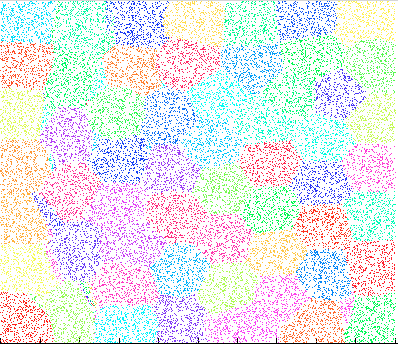
\includegraphics[width=0.8\textwidth,height=0.6\textwidth]{Ekmeans57.png}
\caption{Assign and Balance-EKmeans on 300,000 random 2D points, K= 57 (best seen electronically).}
\label{fig:ekmeans}
\end{minipage}
\hspace{0.08cm}
\begin{minipage}[b]{0.47\linewidth}
\centering
  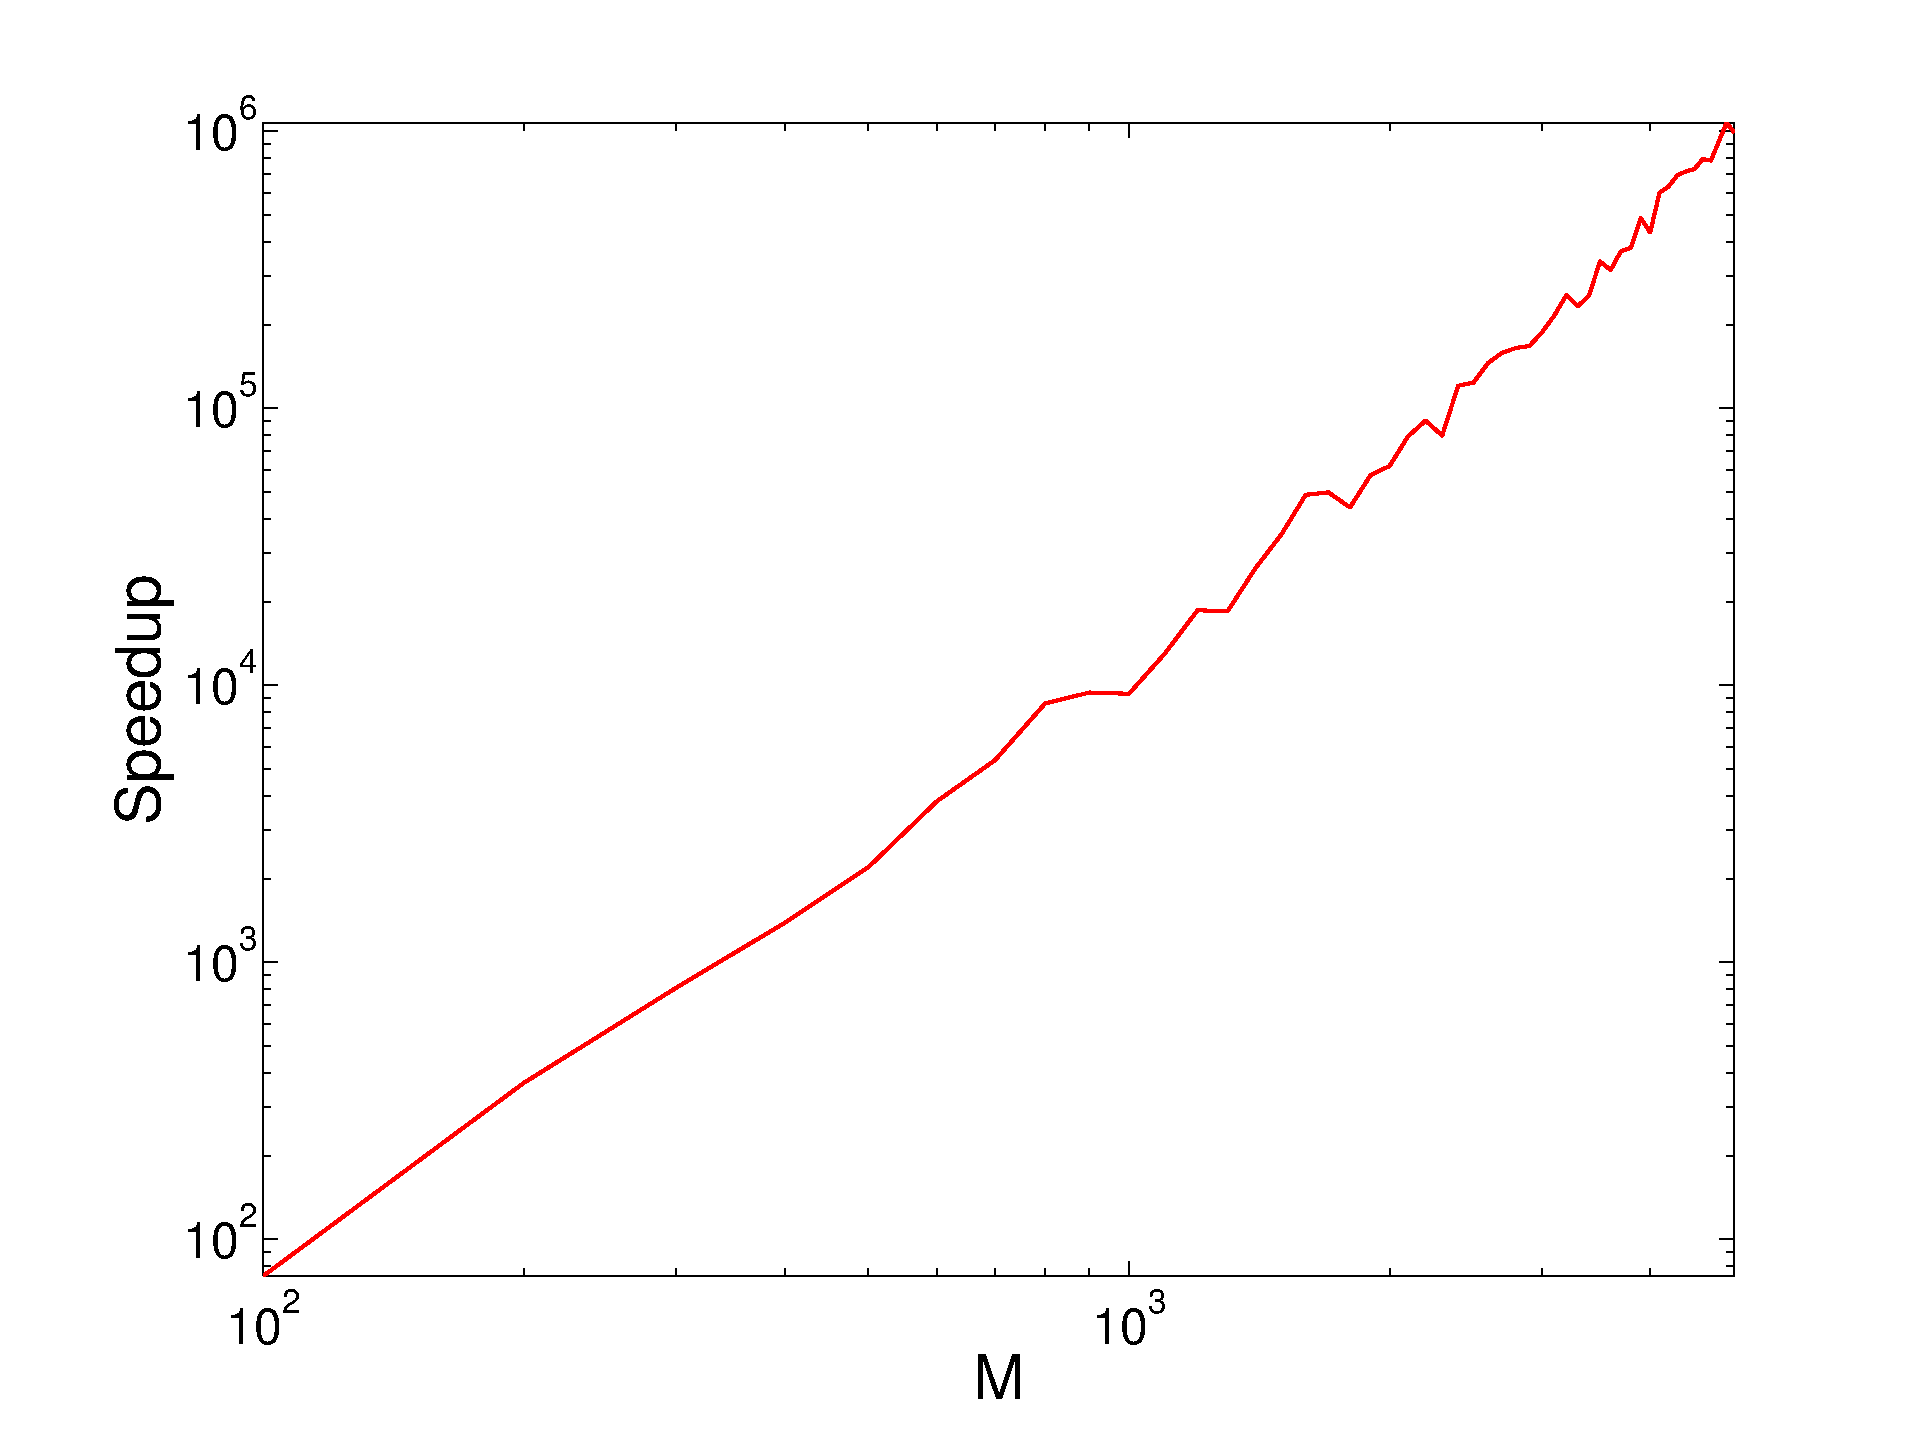
\includegraphics[width=0.7\textwidth,height=0.5\textwidth]{figMInvSpeedUp.eps}
  \vspace{-3mm}
  \caption{Speedup of ODC framework prediction on either TGP or GPR while retrieving precomputed matrix inverses as $M$ increases, compared with computing them on test time by KNN scheme (log-log scale)}
  \label{fig:SpeedUp}
\end{minipage}
\vspace{-6mm}
\end{figure}

an Overlapping Domain Cover (ODC), $\mathcal{D} =  \{ {D}_i: |{D}_i| =M, i=1:K \}$, such that  $D_i \subset X$, $\bigcup_{i} \mathcal{D}_i = X$, and $M$ is the number of points in each subdomain, $|.|$ is the length operator. We assume that the generated subdomains overlaps with other  subdomains in $p \cdot M$ points, such that $0 \le p \le 1$ is the ratio of points in each subdomain that also belongs to/overlaps other subdomains. In our framework, the ODC is based on  with a set of non-overlapping clusters of the data  $C=\{C_1, \cdots, C_K\}$, such that ${D}_i = C_i \cup O_i, \forall i$, $O_i  = \{p_j^i, p_j \in  \{\cup_{j \neq i} \mathcal{C}_j\}$,  $|O_i| = p \cdot M$, $|C_i| = (1-p) \cdot M$.   




, i.e., $|D_i \bigcap \{\cup_{j \neq i} \mathcal{D}_j\} |   = p \cdot M$ and $|D_i \setminus  \{\cup_{j \neq i} \mathcal{D}_j\} |   = (p-1) \cdot M$.  

\end{comment}

  
\begin{comment}
\begin{figure}
\centering
\begin{minipage}[b]{0.6\linewidth}
    \includegraphics[width=1.0\textwidth]{systemArch.png}
  \caption{Domain Decomposition Prediction Framework with pose instances taken from Human Eva dataset  \cite{SigalBB10} }
  \label{fig:DDTGP}
\end{minipage}
\begin{minipage}[b]{0.05\linewidth}
       \begin{tabular}{ccc}
       \end{tabular}              
\end{minipage}
\begin{minipage}[b]{0.2\linewidth}
\begin{tabular}{ccc}
\bmvaHangBox{\fbox{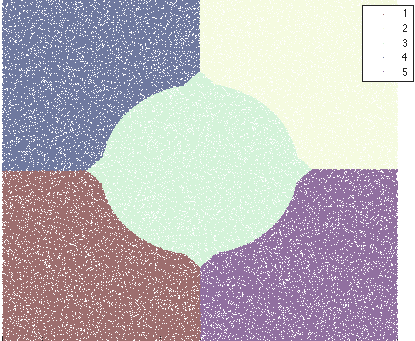
\includegraphics[width=0.6\textwidth]{Ekmeans5}}} \\
(a) 5 clusters \\
\bmvaHangBox{\fbox{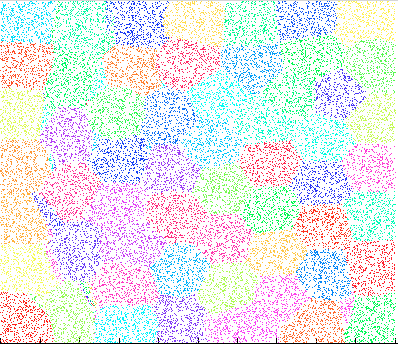
\includegraphics[width=0.7\textwidth]{Ekmeans57}}}\\
(b) 57 clusters \\
\\
\end{tabular}
\caption{EqKmeans of 300,000 random 2D points}
\label{fig:ekmeans}
\end{minipage}
\end{figure}
\end{comment}
\ignore{\begin{figure}[h!]
\centering
\includegraphics[width=0.45\textwidth]{systemArch.png}
  \caption{[TO BE UPDATED OR REMOVED] Overlapping Domain Cover applied to 3D-pose estimation with pose instances taken from Human Eva dataset  \cite{SigalBB10} }
  \label{fig:DDTGP}
\end{figure}}


\begin{comment}
In order to make this notion more concrete, we present the prediction framework in Figure ~\ref{fig:DDTGP}.}

 Training is done by clustering the data and creating consistent subdomains from this data. Then a kernel machine (e.g. TGP, GPR, IWTGP) is created for each of these subdomains.  We denote cluster information and the local kernel machines for the subdomains as ODC Model. During prediction, closest clusters for the test data are retrieved\ignore{ based on different modes ( detailed in next sections \ignore{~\ref{sec:pred})}}. Afterwards ( as an optional phase), the submodels are weighted to handle data bias of the training data. We denote $CovFlag$ as a control flag that enables this phase \footnote{Note that IWTGP is equivalent to TGP if $W  = I$, $I$ is the identity matrix}. Eventually, the final predictions are made by combining the outputs of these subdomain models.
 
 
Our framework configuration starts by specifying two parameters $M$ and the ratio of overlapping points for each subdomain $p$, such that 0$ \le p \le 1$. For each subdomain  $p M$ of the points overlap with other subdomains. 
\end{comment}

